\documentclass{article}
\usepackage{geometry}
 \geometry{
 a4paper,
 total={210mm,297mm},
 left=20mm,
 right=20mm,
 top=20mm,
 bottom=20mm,
 }

\usepackage{siunitx} % Provides the \SI{}{} command for typesetting SI units
\usepackage{listings}
\usepackage{graphicx} % Required for the inclusion of images
\usepackage{enumerate}
\usepackage{float}
\usepackage{fancyvrb}
\usepackage[utf8]{inputenc}
\usepackage{listings}
\usepackage{inconsolata}
\usepackage{placeins}
\usepackage{subcaption}
\usepackage[draft]{fixme}

\usepackage{hyperref}
\hypersetup{
  colorlinks   = true,    % Colours links instead of ugly boxes
  urlcolor     = blue,    % Colour for external hyperlinks
  linkcolor    = blue,    % Colour of internal links
  citecolor    = red      % Colour of citations
}

\newcommand{\codelink}[1]{%
    \hyperref[#1]{Matlab Code (Listing~\ref{#1})}%
}

\lstset{
    frame=single,
    basicstyle=\small\ttfamily,
    language=bash
}

\setlength\parindent{0pt} % Removes all indentation from paragraphs

\title{Network Security \\ 389.159 - SS 2018 \\ Lab Exercise 3 \& Lab Exercise 4} % Title

\author{
    TEAM 02 \\
    Corentin \textsc{Bergès} (11741629) (066 506) \\
    Christoph \textsc{Echtinger-Sieghart} (00304130) (066 938)
}

\date{\today} % Date for the report
\begin{document}

\maketitle % Insert the title, author and date
\renewcommand{\arraystretch}{2} %Stretch rows

\listoffixmes

\section{Lab Exercise 3}

\subsection{rep-10 }

\codelink{code:rep-10}

Figure~\ref{figure:rep-10} shows the stem plots for packets, bytes, IP sources and IP destinations
per hour.

\begin{figure}[h]
    \begin{subfigure}{.5\textwidth}
        \centering
        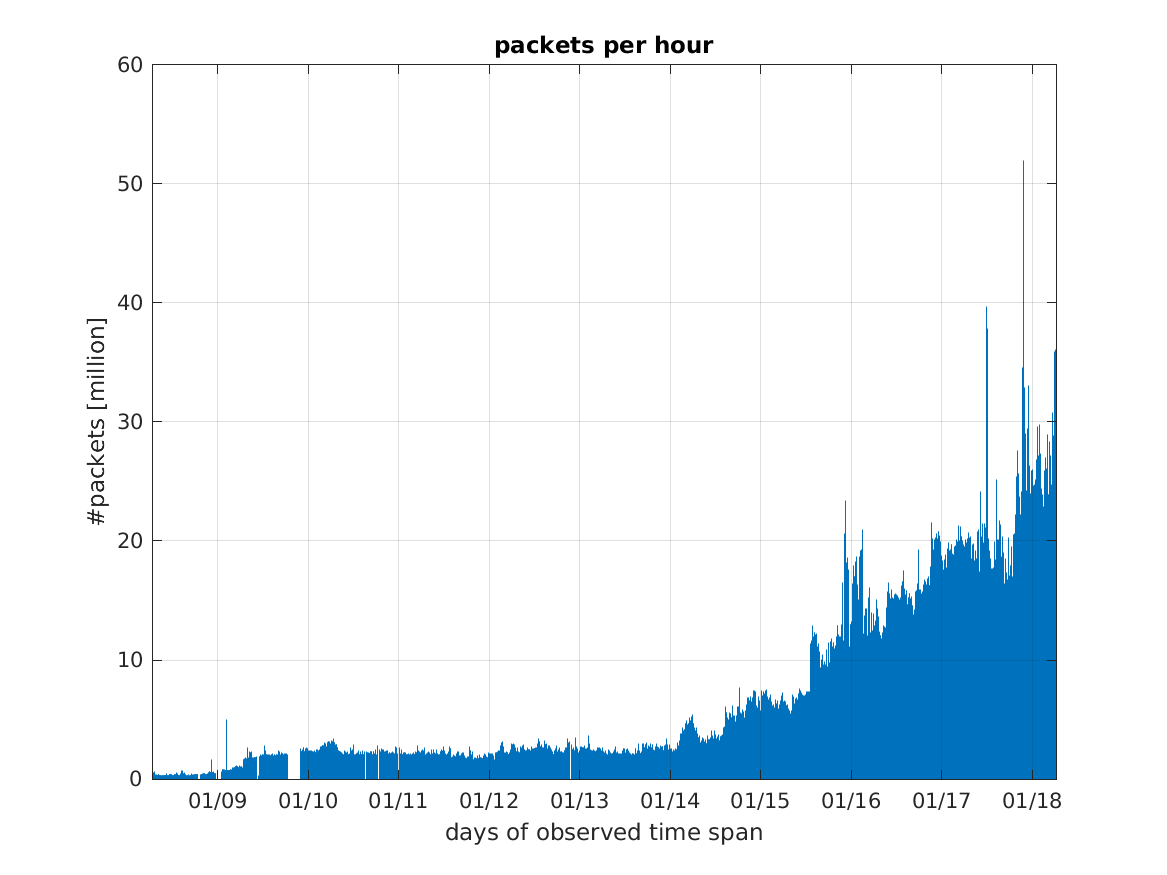
\includegraphics[width=\textwidth]{../exercise-3/plots/rep_10_1}
        \caption{Packets per hour}
    \end{subfigure}
    \begin{subfigure}{.5\textwidth}
        \centering
        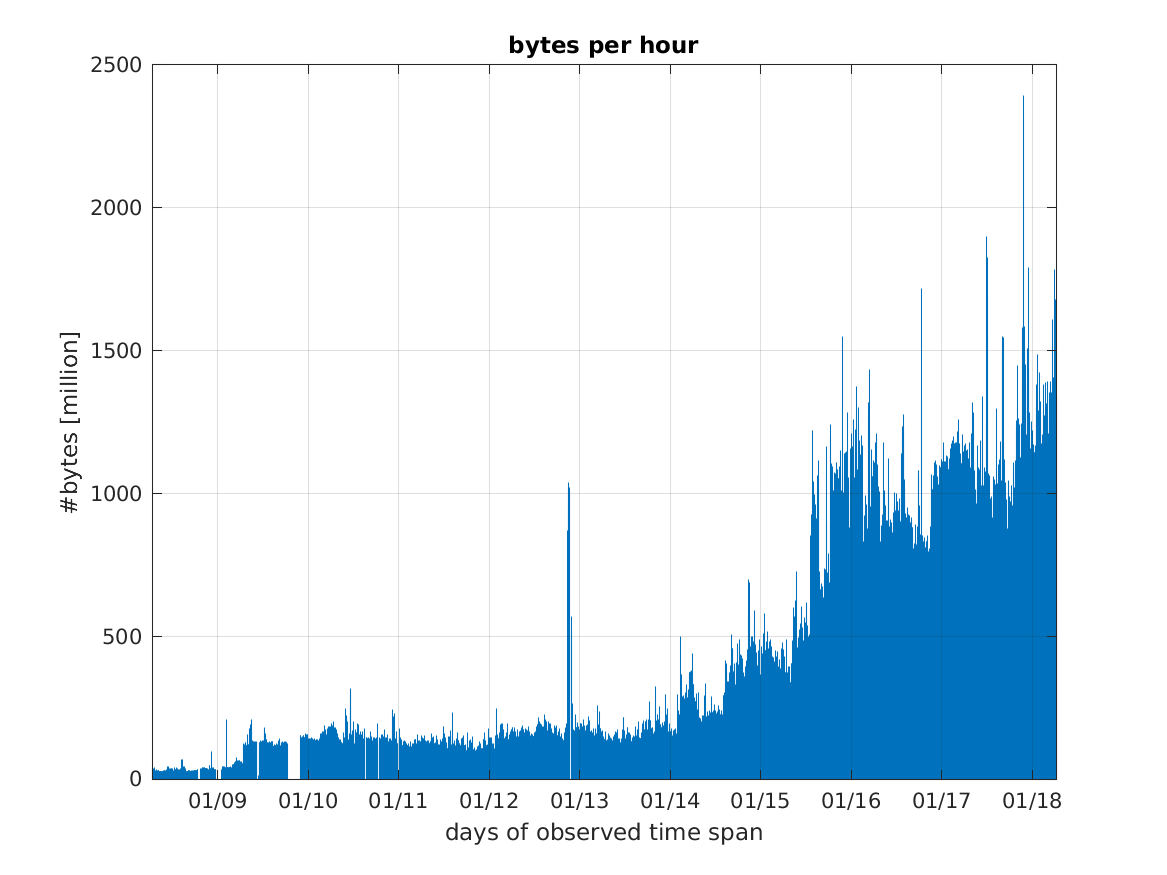
\includegraphics[width=\textwidth]{../exercise-3/plots/rep_10_2}
        \caption{Bytes per hour}
    \end{subfigure}
    \begin{subfigure}{.5\textwidth}
        \centering
        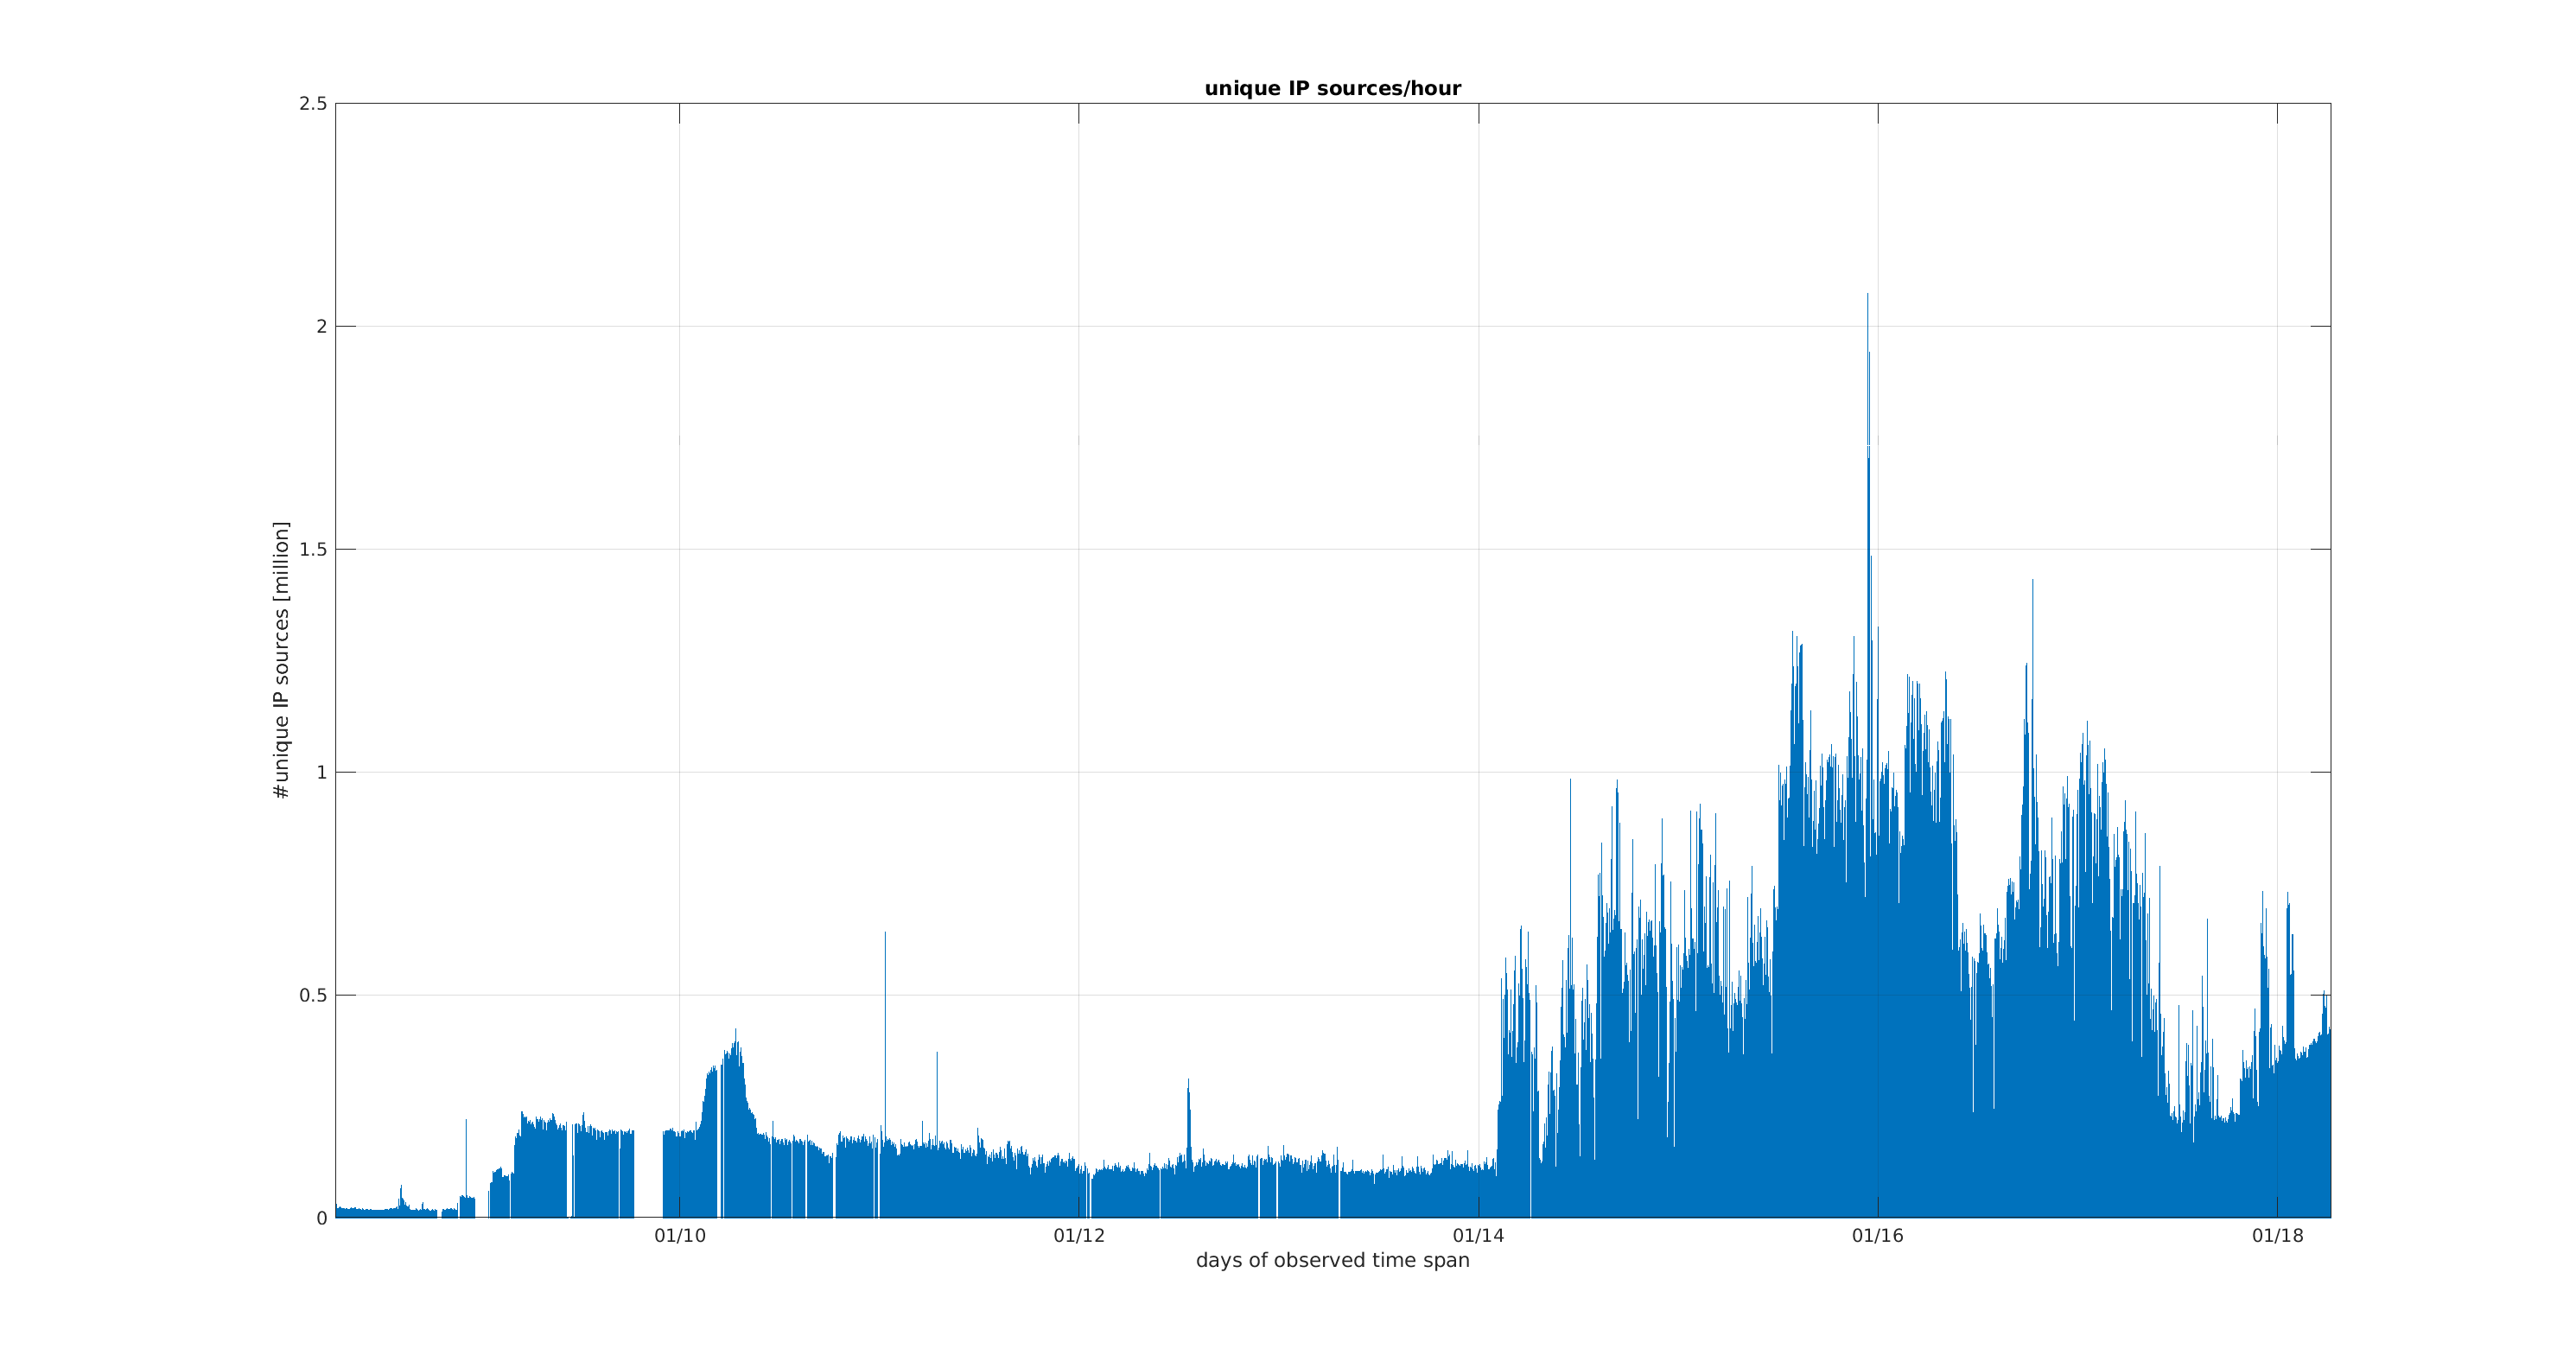
\includegraphics[width=\textwidth]{../exercise-3/plots/rep_10_3}
        \caption{IP sources per hour}
    \end{subfigure}
    \begin{subfigure}{.5\textwidth}
        \centering
        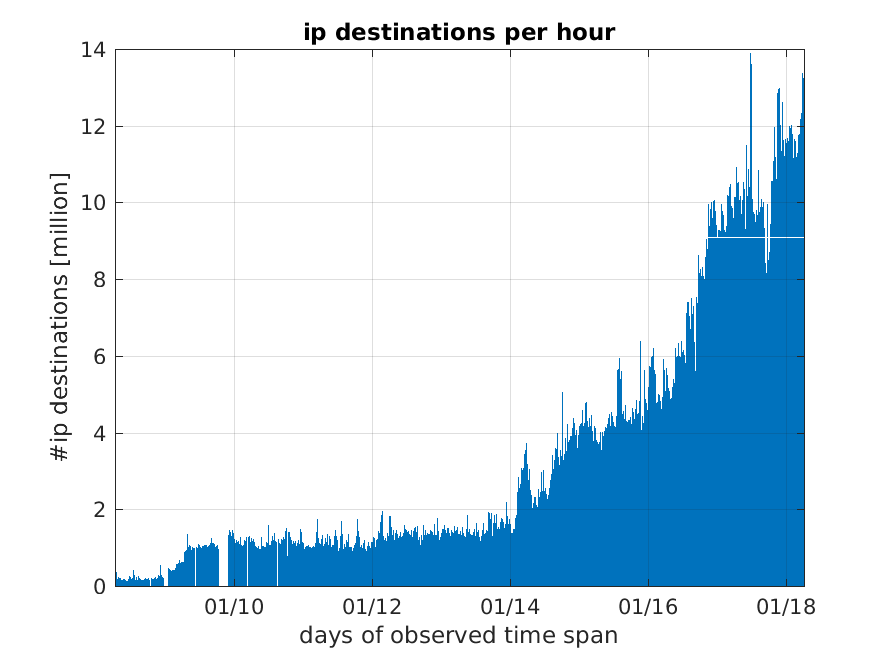
\includegraphics[width=\textwidth]{../exercise-3/plots/rep_10_4}
        \caption{IP destinations per hour}
    \end{subfigure}
    \caption{\label{figure:rep-10}}
\end{figure}

\paragraph{Optional}

Figure~\ref{figure:rep-10-optional} shows all signals from Figure~\ref{figure:rep-10} combined, normalized
and smoothed with a moving average filter.

\begin{figure}[h]
    \centering
    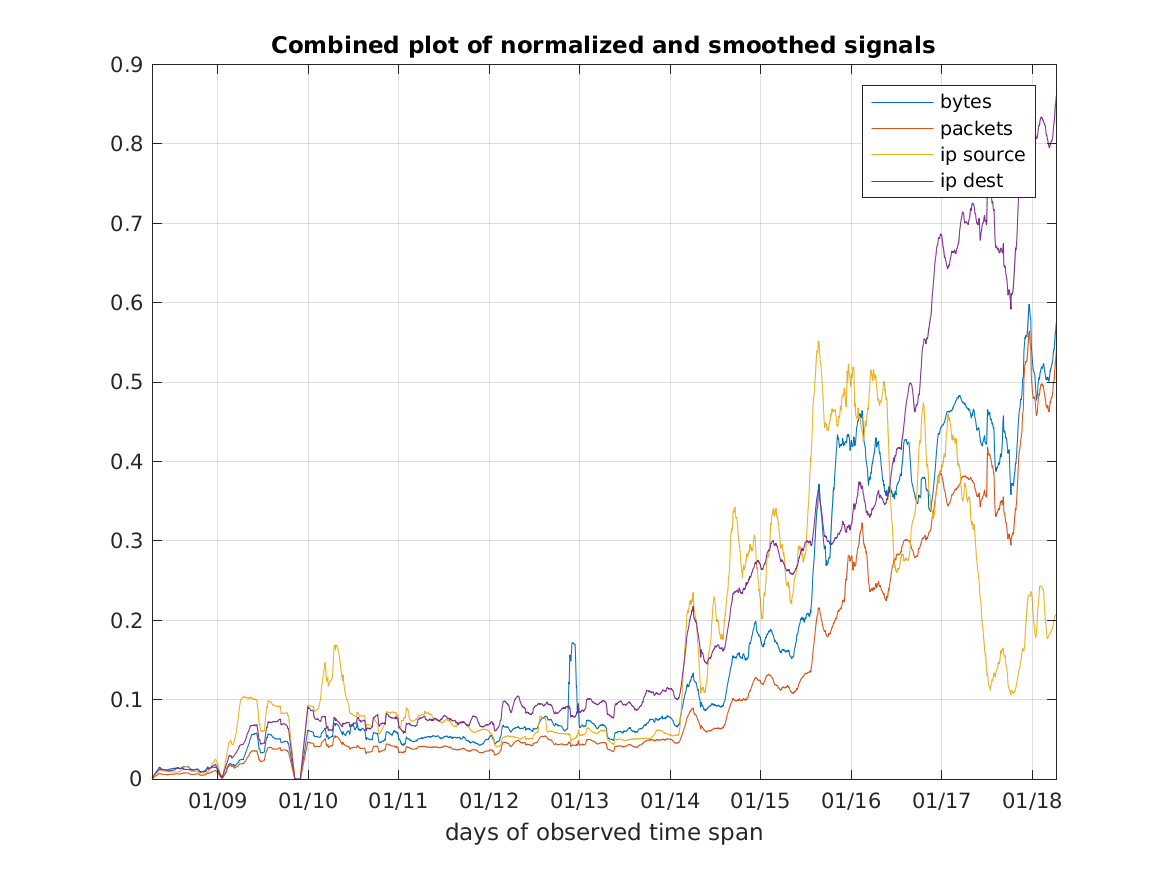
\includegraphics[width=\textwidth]{../exercise-3/plots/rep_10_optional}
    \caption{\label{figure:rep-10-optional} Combined, normalized and smoothed signals}
\end{figure}

\subsection{rep-11}

\codelink{code:rep-11}

The signal that shows the lower correlation to the other signals is \textbf{IP sources}. The minimum
linear correlation coefficient is \textbf{0.588568} between the signals \textbf{IP sources} and
\textbf{IP destinations}. See Table~\ref{table:rep-11} for the raw data.

\fxerror{Include row descriptions and expand}

\begin{table}[h]
    \centering
    \begin{tabular}{c|c|c|c}
        Bytes & Packets & IPs & IPd \\
        \hline
        0.9655 &   0.9655 &   0.7203 &   0.9340 \\
        0.7203 &   0.6105 &   0.6105 &   0.9732 \\
        0.9340 &   0.9732 &   0.5886 &   0.5886 \\
    \end{tabular}
    \caption{\label{table:rep-11} Correlation coefficients between signals}
\end{table}

\fxerror{Answer question}
The reason why the drop in unique IP sources does not cause a proportional drop ...

\subsection{rep-12}

\codelink{code:rep-12}


\fxerror{Wording!}
There are around ten times more IP sources than IP destinations. It makes sense that the
number of IP sources is significantly bigger than the number of IP destinations because the
darkspace is only a part of the whole internet.

\subsection{rep-13}
\codelink{code:rep-13}

The main peak in IP sources starts at 14-Dec-2015 and lasts until 16-Dec-2015. See Table~\ref{table:rep-13}
for the detailed data.

\begin{table}[h]
    \centering
    \begin{tabular}{cr}
        Date & \# IP sources \\
        \hline
        14-Dec-2015 & 2075358.074306 \\
        15-Dec-2015 & 1704892.012500 \\
        16-Dec-2015 & 1942072.404167 \\
    \end{tabular}
    \caption{\label{table:rep-13} Detailed data for peak in IP sources}
\end{table}

\paragraph{Optional}
\codelink{code:rep-13-optional}
The main peak in Bytes starts at 14-Nov-2012 and lasts until 22-Nov-2012. Note that
on 19-Nov-2012 no data was available. See Table~\ref{table:rep-13-optional}
for the detailed data.

\begin{table}[h]
    \centering
    \begin{tabular}{cr}
        Date & \# Bytes \\
        \hline
        14-Nov-2012& 870858582.136110 \\ 
        15-Nov-2012& 1009586335.331900 \\
        16-Nov-2012& 1038654926.456100 \\
        17-Nov-2012& 1021464983.022200 \\
        18-Nov-2012& 954193481.914190 \\ 
        20-Nov-2012& 1005163238.508500 \\
        21-Nov-2012& 1020526661.658000 \\
        22-Nov-2012& 989613880.615110  \\
    \end{tabular}
    \caption{\label{table:rep-13-optional} Detailed data for peak in Bytes}
\end{table}

\subsection{rep-14}
\codelink{code:rep-14}

Table~\ref{table:rep-14-daily} gives statistics for the data from
\texttt{global\_last10years.csv}. Table~\ref{table:rep-14-hourly} gives
statistics for the data from \texttt{Feb2017\_gen.csv}.

\begin{table}[h]
    \centering
    \begin{tabular}{l|rrrr}
                & Sum & Mean & Median & StdDev \\
                \hline
        \# Packets &   146373.391 & 41.845 & 17.699 & 40.916 \\
        \# Bytes   &    2381.003 & 0.681 & 0.263 & 0.735 \\
        \# IP src     & 123.613 & 0.035 & 0.020 & 0.031 \\
        \# IP dst     & 1150.796 & 0.329 & 0.142 & 0.330 \\
    \end{tabular}
    \caption{\label{table:rep-14-daily} Statistics for daily data [in millions]}
\end{table}

\begin{table}[h]
    \centering
    \begin{tabular}{l|rrrr}
                & Sum & Mean & Median & StdDev \\
                \hline
        \# Packets &    76871.319 & 114.392 & 113.464 & 7.033 \\
        \# Bytes   &    1272.998  &1.894 & 1.890 & 0.097      \\
        \# IP src     & 59.651 & 0.089 & 0.091 & 0.018        \\
        \# IP dst     & 619.875 & 0.922 & 0.931 & 0.070       \\
    \end{tabular}
    \caption{\label{table:rep-14-hourly} Statistics for hourly data [in millions]}
\end{table}

\subsection{rep-15}

The values do not coincide. Feb2017 seems to be a month that is not really representative for the
whole span of 10 years.

% + optional

\paragraph{optional}

\codelink{code:rep-15-optional}

\begin{figure}[h]
    \centering
    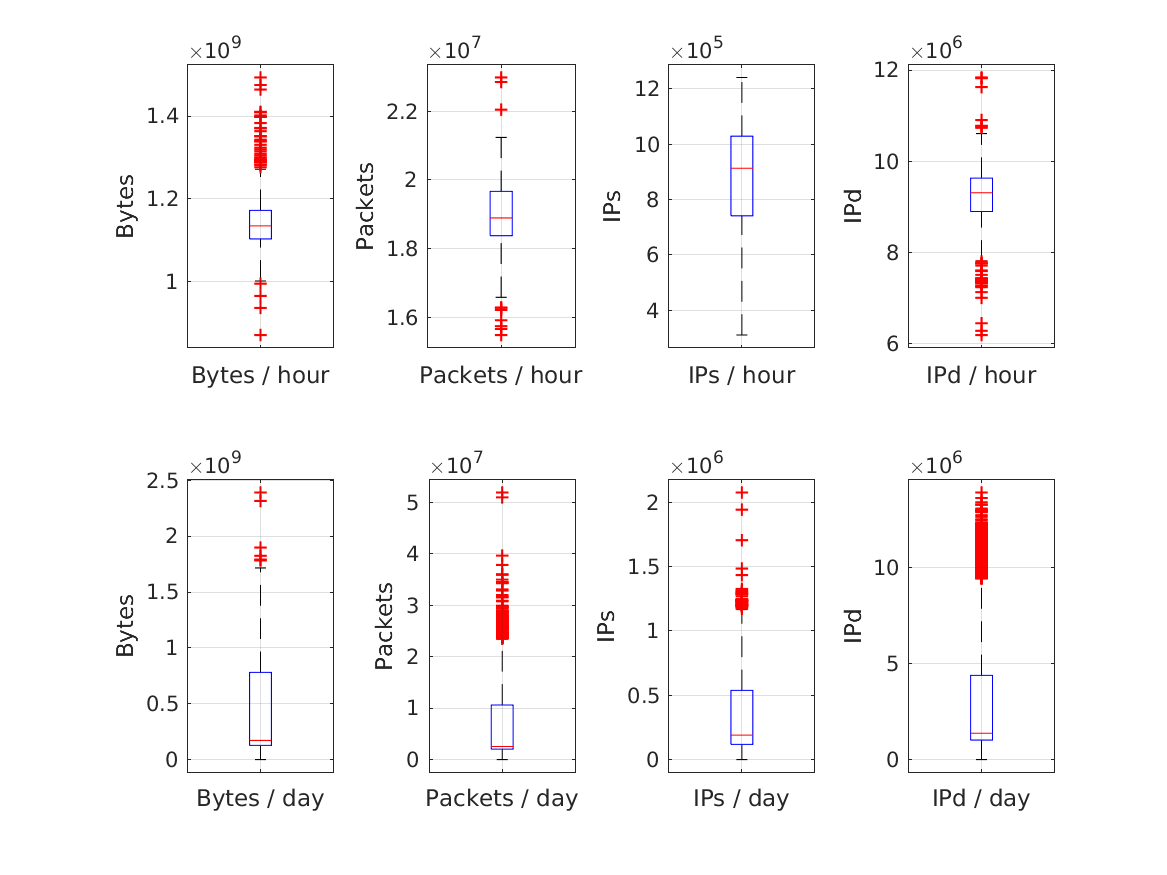
\includegraphics[width=\textwidth]{../exercise-3/plots/rep_15_optional}
    \caption{\label{figure:rep-15-optional} Boxplots for hourly and daily averaged data}
\end{figure}

\subsection{rep-16}

We used https://www.iana.org/assignments/protocol-numbers/protocol-numbers.xhtml to look up the
protocol numbers.

\paragraph{Protocol 6 (TCP)}
The Transmission Control Protocol
\fxerror{tcp}
\paragraph{Protocol 1 (ICMP)}
The Internet Control Message Protocol
\fxerror{icmp}
\paragraph{Protocol 17 (UDP)}
The User Datagram Protocol
\fxerror{udp}

\subsection{rep-17}
% + optional
\subsection{rep-18}

\fxerror{Wording}
We obtained negative values because of collapsing ...

%optional
\subsection{rep-19}

%optional
\subsection{rep-20}

\subsection{rep-21}
\subsection{rep-22}
\subsection{rep-23}

\begin{lstlisting}[label=listing:ip-command,caption={Command used to obtain IP address}]
team02@pc01:~$ ip address show dev em1
\end{lstlisting}

\paragraph{Port 113}
\begin{Verbatim}
IP 192.168.83.20.1073 > 192.168.83.33.113: Flags [S], seq 0, win 8192, length 0
IP 192.168.83.33.113 > 192.168.83.20.1073: Flags [R.], seq 0, ack 1, win 0, length 0
\end{Verbatim}

\section{Lab Exercise 4}

\subsection{rep-24}
\subsection{rep-25}
\subsection{rep-26}
\subsection{rep-27}
\subsection{rep-28}
\subsection{rep-29}
\subsection{rep-30}

\FloatBarrier

\appendix
\newpage
\section{Matlab Code}
\lstinputlisting[%
    float,language=Matlab,caption={Matlab code to solve rep-10},label=code:rep-10%
]{../exercise-3/team02_rep10.m}

\lstinputlisting[%
    float,language=Matlab,caption={Matlab code to solve rep-11},label=code:rep-11%
]{../exercise-3/team02_rep11.m}

\lstinputlisting[%
    float,language=Matlab,caption={Matlab code to solve rep-12},label=code:rep-12%
]{../exercise-3/team02_rep12.m}

\lstinputlisting[%
    float,language=Matlab,caption={Matlab code to solve rep-13},label=code:rep-13%
]{../exercise-3/team02_rep13.m}

\lstinputlisting[%
    float,language=Matlab,caption={Matlab code to solve rep-13 optional},label=code:rep-13-optional%
]{../exercise-3/team02_rep13_optional.m}

\lstinputlisting[%
    float,language=Matlab,caption={Matlab code to solve rep-14},label=code:rep-14%
]{../exercise-3/team02_rep14.m}

\lstinputlisting[%
    float,language=Matlab,caption={Matlab code to solve rep-15 optional},label=code:rep-15-optional%
]{../exercise-3/team02_rep15_optional.m}

\end{document}
